% Add this to the preamble if it is not already present:
% \usepackage{graphicx}

\begin{figure}[htbp]
\centering
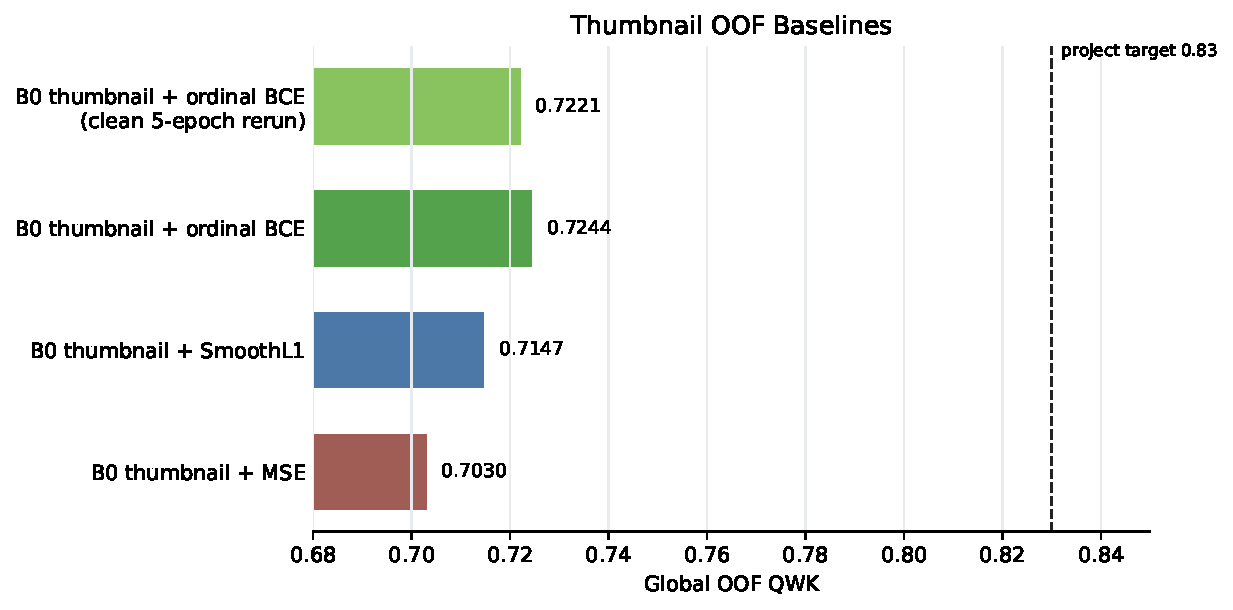
\includegraphics[width=0.9\textwidth]{graphics/qwk_oof_model_comparison.pdf}
\caption{Global out-of-fold QWK for the main thumbnail baselines. Ordinal BCE is the strongest current thumbnail setup, but remains below the target QWK of 0.83.}
\label{fig:qwk-oof-model-comparison}
\end{figure}

\begin{figure}[htbp]
\centering
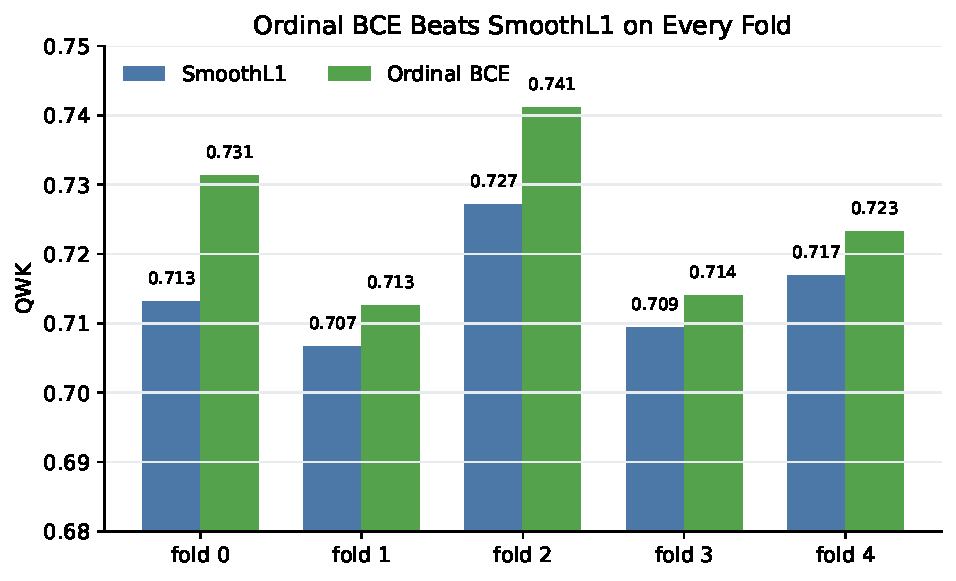
\includegraphics[width=0.9\textwidth]{graphics/fold_qwk_smoothl1_vs_ordinal.pdf}
\caption{Per-fold QWK comparison between the recovered SmoothL1 and ordinal BCE OOF predictions. Ordinal BCE improves over SmoothL1 on every fold.}
\label{fig:fold-qwk-smoothl1-vs-ordinal}
\end{figure}

\begin{figure}[htbp]
\centering
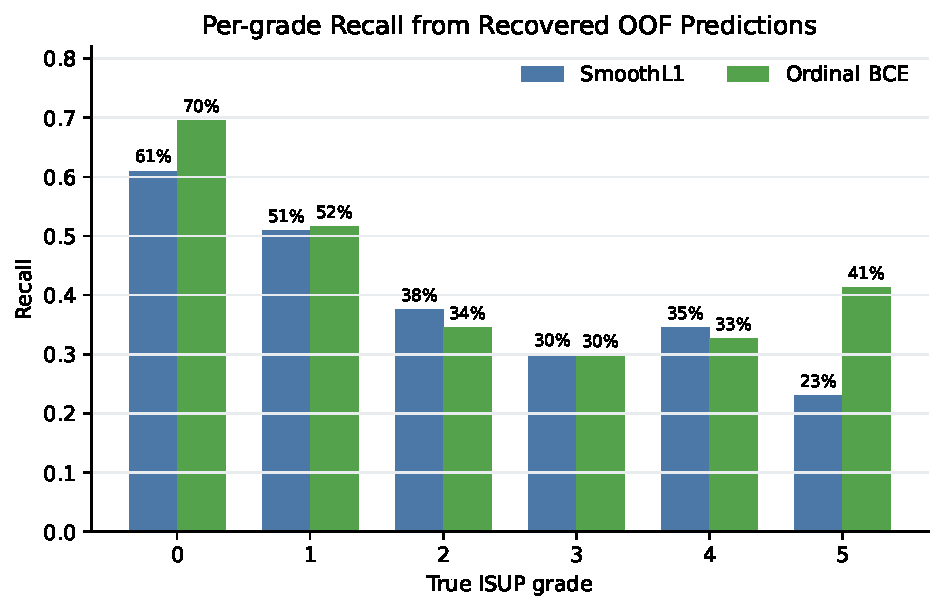
\includegraphics[width=0.9\textwidth]{graphics/isup_recall_smoothl1_vs_ordinal.pdf}
\caption{Per-grade recall for the recovered SmoothL1 and ordinal BCE OOF predictions. Ordinal BCE improves recall for the clinically important extreme grades, especially ISUP 5.}
\label{fig:isup-recall-smoothl1-vs-ordinal}
\end{figure}

\begin{figure}[htbp]
\centering
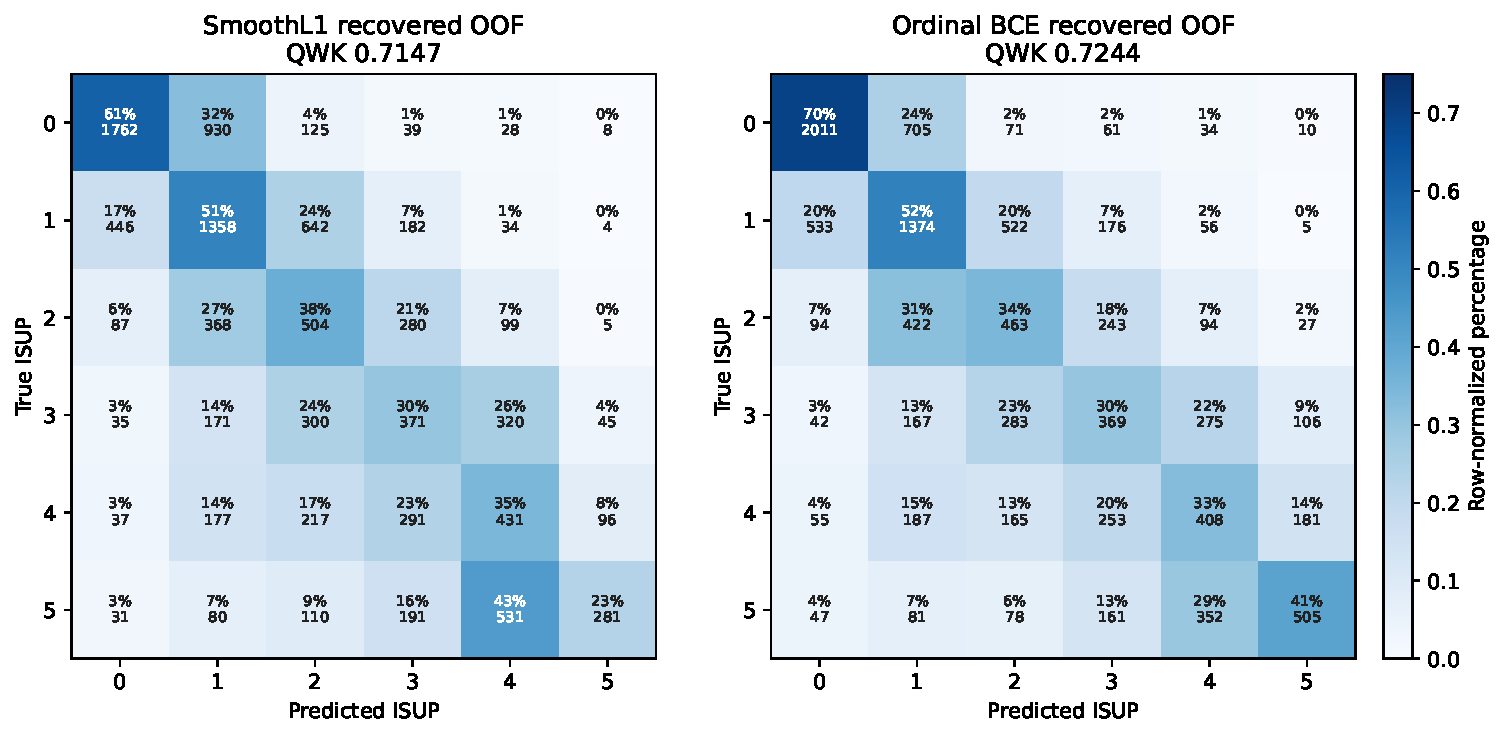
\includegraphics[width=\textwidth]{graphics/confusion_matrices_smoothl1_vs_ordinal.pdf}
\caption{Row-normalized confusion matrices for recovered SmoothL1 and ordinal BCE OOF predictions. Each cell shows row percentage and slide count.}
\label{fig:confusion-smoothl1-vs-ordinal}
\end{figure}

\begin{figure}[htbp]
\centering
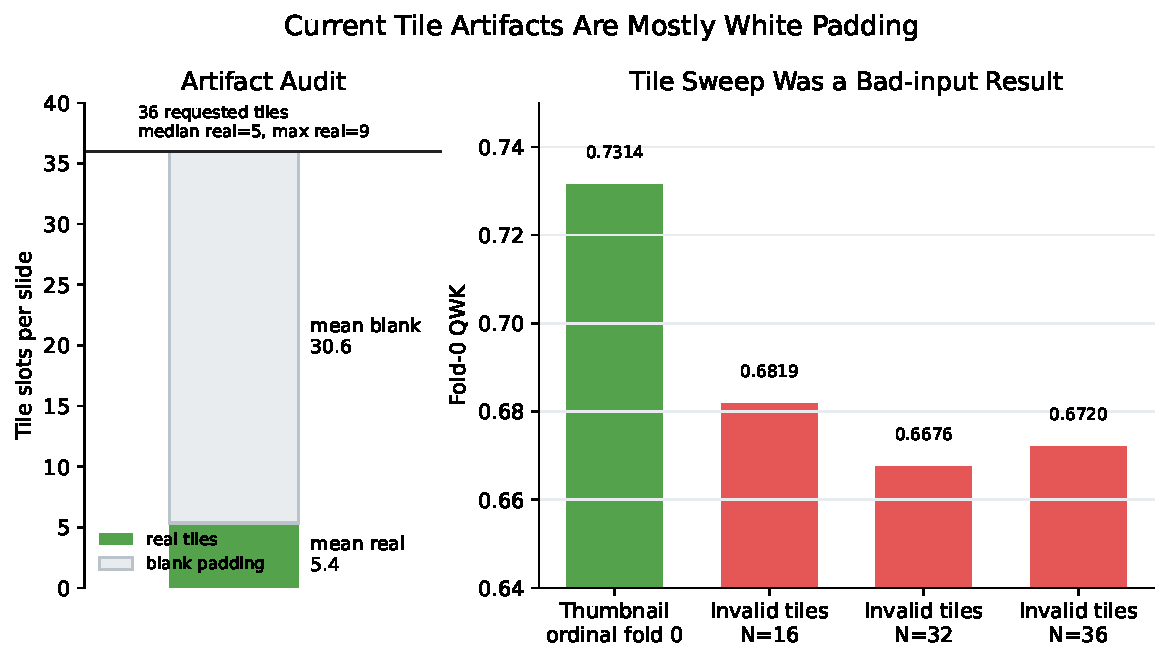
\includegraphics[width=0.95\textwidth]{graphics/tile_artifact_audit.pdf}
\caption{Tile artifact audit and fold-0 tile sweep. The current 36-tile artifacts contain only about five real tissue tiles per slide on average, so the tile sweep should be interpreted as a bad-input result rather than evidence against tile-based modeling.}
\label{fig:tile-artifact-audit}
\end{figure}

\begin{figure}[htbp]
\centering
\includegraphics[width=0.72\textwidth]{graphics/invalid_tile_artifact_example.png}
\caption{Example of the current 36-tile artifact format. Green outlines mark estimated tissue-containing tiles; the remaining slots are blank or near-blank padding.}
\label{fig:invalid-tile-artifact-example}
\end{figure}
